%!TEX root = iclr2026_conference.tex
% Granularity storyline (2026-09-26): §3 formalizes the Introduction's three innovations; §4 implements them.
% Constants trace to the read-only NovPhy
% code (paths relative to the NovPhy repository root): world_model/training/cnn_hybrid.py (CH),
% world_model/model/predictor.py (PR), world_model/training/matched_dynamics.py (MD),
% scripts/run_issue_77_n1_train.py (N1T), world_model/planning/task_objective.py (TO),
% .local-artifacts/issue-77-n1-dynamics-v1/plan.json (N1P).
% \varnothing needs amssymb, which the preamble does not load (math_commands.tex loads amsmath/amsfonts only);
% fall back to \emptyset so this file compiles either way. No-op once amssymb is loaded.
\providecommand{\varnothing}{\emptyset}
% ==== BRIEF §3 HEAD (Problem Formulation) =============================================
% [中] 定位：把 Intro 的三条创新写成形式对象：(1) 动作稀疏 MDP 与无需中间动作的 Δ 步核；(2) 同一共享潜变量上的预测请求
%      r=(Δ,α)；(3) 请求选择问题（误差与计算的权衡目标），其解法留给 §4；最后把预测接到决策上：候选排序、引擎结局 y、排序 AUC，
%      以及同一 checkpoint 上"逐预测选择 vs 固定请求"的比较。
% 卖点：环境仍是普通 MDP；粒度是模型每次预测的请求，与动作分开。
%      主张：动作稀疏使 Δ 步跳跃良定义；所有请求由同一预测器在同一 236 维 carrier 空间中服务；请求策略的目标是时长加权的
%            预测误差加归一化计算量。
%      证据：CH:18-22（PAIRS、DIM=236）；CH:75-86（谓词回馈）；CH:142-155（Δ>剩余帧掩码）；CH:158-176（linear_macs）；
%            CH:179-212（trajectory_labels 代价与递推）；CH:216-239（adaptive_rollout）；N1T:14-19（N1 帧距 50 引擎步）；
%            TO:31-42（计数代价）；scripts/run_tau_ad_within_checkpoint.py:1-16（所有臂同一 checkpoint、同一端点 225、同一代价）。
%      手法/边界：定义用陈述句，每个符号首用即定义，编号公式。边界：本节无结果数字；不写两轴必须一起选；不写选择粒度有益；
%            目标只在训练轨迹上有定义；策略只在 decision-only 想象 rollout 中评估（§5 写明）。
% [EN] Role: turns the Introduction's three innovations into formal objects: (1) the action-sparse MDP and the Δ-step
%      kernel that needs no intermediate actions; (2) prediction requests r = (Δ, α) on one shared latent; (3) the
%      request-selection problem (error-versus-compute objective), solved in Section 4; then connects predictions to
%      decisions: candidate ranking, engine outcome y, ordering AUC, and the per-prediction versus fixed-request
%      comparison on one checkpoint.
% Pitch: the environment stays an ordinary MDP; granularity is a request attached to every model prediction.
%      Evidence: code lines as listed above.
%      Craft/Boundaries: declaratives, symbols defined at first use, numbered equations. No result numbers; never "the
%      axes must be chosen together"; no benefit claim; the objective exists on training trajectories only; the policy
%      was evaluated only in decision-only imagined rollouts (stated in Section 5).
% ==== /BRIEF ==========================================================================
\section{Problem Formulation}
\label{sec:mth:setting}

% ==== BRIEF §3 ¶1 (action-sparse MDP and the Δ-step kernel) ============================
% [中] 定位：创新 1 的形式基础。给出环境类（引擎步 MDP + 空动作 + 稀疏决策步），再写出两个决策步之间的 n 步转移核：
%      只依赖当前状态与该步起点的动作，不需要中间动作；因此预测可跳任意步数，环境仍是普通 MDP。一句带过 PHYRE 的 bandit 框定。
%      主张：M=(S, A∪{∅}, P, R)；a_t≠∅ 仅在决策步；P^n 为 P 与 ∅ 的复合；NovPhy 中动作是一次弹弓发射（含其内部安排的 tap）。
%      证据：CH 与 N1T 的决策契约（一次发射后自主级联；world_model/data/deployment_temporal.py:219-303）；
%            bakhtin2019phyre 的 contextual-bandit 原文表述（Intro ¶2 已引）。
%      手法与边界：公式后一句读法；不写"MDP 变体"；不说 PHYRE 错误；环境类本身不是贡献。
% [EN] Role: formal basis of innovation 1: the environment class, then the n-step kernel between decision steps, which
%      depends on the current state and the action at its start only; a prediction can therefore jump any number of
%      steps and the environment stays an ordinary MDP. One clause on PHYRE's bandit framing.
%      Evidence: the decision contract in CH and N1T; PHYRE's contextual-bandit framing (cited in the Introduction).
%      Craft/Boundaries: equation, then its reading; never "an MDP variant"; never call PHYRE wrong.
% ==== /BRIEF ==========================================================================
An action-sparse persistent-effect environment is a Markov decision process $\mathcal{M}=(\mathcal{S},\mathcal{A}\cup\{\varnothing\},P,R)$ over engine steps $t$, where $\varnothing$ is the null action, $R$ is the task reward, and actions are sparse:
\begin{equation}
s_{t+1}\sim P(\cdot\mid s_t,a_t),\qquad a_t\neq\varnothing\ \text{only if}\ t\in\mathcal{T}_{\mathrm{dec}},
\label{eq:mdp}
\end{equation}
with $\mathcal{T}_{\mathrm{dec}}$ the small set of decision steps. In NovPhy an action is one slingshot launch, and the agent observes an RGB frame $o_t$. Because the agent issues no further action between decision steps, the state $n$ steps ahead depends only on the current state and the action taken there, provided no decision step lies in $(t,t+n)$:
\begin{equation}
P^{n}(s_{t+n}\mid s_t,a_t)=\int P(s_{t+1}\mid s_t,a_t)\prod_{\tau=t+1}^{t+n-1}P(s_{\tau+1}\mid s_\tau,\varnothing)\,\mathrm{d}s_{t+1:t+n-1}.
\label{eq:kernel}
\end{equation}
A prediction may therefore jump any number of steps without intermediate actions, and $\mathcal{M}$ remains an ordinary MDP. Treating the launch as the only decision would instead fold the cascade into the outcome of $(s,a)$, the contextual-bandit framing of PHYRE \citep{bakhtin2019phyre}; we keep the cascade and let the model decide how to predict it.

% ==== BRIEF §3 ¶2 (prediction requests on one shared latent) ==========================
% [中] 定位：创新 2 的形式基础。定义 carrier、carrier 帧、请求空间 R 与 Δ、α 的含义；说明 α 通过谓词回馈改变被推进的内容；
%      所有请求由同一预测器服务并返回同一 236 维空间中的 carrier，故 rollout 可在任意一步换请求。
%      主张：三个描述层各给一个具体含义与例子（cont：每个物体的存在、类别、位置、速度；micro：成对的 contact 与 supports；
%            macro：steady-state 与 structure-unstable 两个场景谓词），并以 Figure fig:levels 的真实帧举例（frame 165：pig–platform0 contact 与 platform0→pig supports；macro 两项均为 0，
%            静止帧 554 steady-state=1）；
%            z=E(o)∈R^236；N1 上一个 carrier 帧 = 50 引擎步；R={1,5,15}×{cont,micro,macro}，|R|=9；ẑ_{k+Δ}=F_θ(ẑ_k,a,r)≈z_{k+Δ}；
%            发射 a 条件化每次预测。
%      证据：CH:44-73（micro_head 输出 18×18×2 的 contact/supports 与 2 个 availability；macro_head 输出 2 个谓词与 2 个
%            availability）；world_model/model/config.py:26-27（MICRO=(contact, supports)，MACRO=(steady-state, structure-unstable)）；
%            CH:18-22（PAIRS、DIM=236）；CH:75-86（adapter 回馈，只在 micro/macro）；N1T:14-19（N1 帧距 50 引擎步）。
%      手法与边界：一式一句；α 不减少潜变量维度，也不只改变读出；单位只对 N1 采集成立（基础语料的单位差异在 §4 披露）。
% [EN] Role: formal basis of innovation 2: carrier, carrier frame, request space and the meaning of Δ and α; α changes
%      what is rolled forward through predicate feedback; one predictor serves every request and returns a carrier in
%      the same 236-d space, so a rollout can change its request at any step.
%      Evidence: CH:18-22; CH:75-86 (adapter feedback for micro/macro only); N1T:14-19 (50 engine steps per N1 frame).
%      Craft/Boundaries: α neither shrinks the latent nor changes only the readout; the unit holds for N1 captures.
% ==== /BRIEF ==========================================================================
A frozen object-slot encoder $E$ maps an observation to the \emph{carrier} $z=E(o)\in\mathbb{R}^{236}$, a continuous latent state (Section~\ref{sec:mth:model}). We index carrier frames by $k$, with $z_k$ the carrier of the $k$-th captured frame after the decision step; on N1 captures one carrier frame spans 50 engine steps. Every world-model query carries a \emph{prediction request}
\begin{equation}
r=(\Delta,\alpha)\in\mathcal{R}=\{1,5,15\}\times\{\textsf{cont},\textsf{micro},\textsf{macro}\},\qquad|\mathcal{R}|=9 .
\label{eq:requests}
\end{equation}
The horizon $\Delta$ is the number of carrier frames the prediction advances. The description level $\alpha$ sets what the prediction reasons over. Under $\textsf{cont}$ (continuous) it is the carrier alone, which lists each object's presence, kind, position and velocity. Under $\textsf{micro}$ it adds relations between pairs of objects: which objects touch and which object supports which. Under $\textsf{macro}$ it adds two predicates of the whole scene: whether the scene has come to rest and whether the structure is unstable. In the scene of Figure~\ref{fig:levels}, $\textsf{micro}$ records that the pig touches the platform beneath it and that this platform supports the pig, while $\textsf{macro}$ records only that the scene is not yet at rest. Under $\textsf{micro}$ and $\textsf{macro}$ the model reads these predicates from its state and feeds them back into the transition, so $\alpha$ changes what is rolled forward. One predictor serves every request and returns a carrier in the same space, $\hat z_{k+\Delta}=F_\theta(\hat z_k,a,r)\approx z_{k+\Delta}$, so a rollout can change its request at any step. The launch $a$ conditions every prediction.

% ==== BRIEF FIG (fig:levels) ====
% [中] 定位：§3 三个描述层的定义性实例，不是模型准确率结果。
%      主张：同一真实画面可描述为物体状态、成对关系及场景谓词。
%      证据：figures/build_description_levels.py；/p/Project/NovPhy/.local-artifacts/ 下
%      issue-77-n1-v1/attempts/issue-77-n1-001-a06/shot-1 的 agent frame_000165.png，
%      native fixed_step=38250；issue-77-n1-dynamics-v1/shards/lineage-n1-001.pt
%      window 25 offset 0（关系/宏标签），window 27 offset 60（frame 554 已稳定对照）。
%      手法与边界：三个面板相同裁剪，连续量由引擎投影，关系/谓词直接读训练张量；不是模型读出。
%      初试 checkpoint issue-77-n1-dynamics-v1/seed-20260908/hybrid/predictor.pt
%      在 teaser a06 frame 80 的冻结解析器 carrier 上没有 gated probability >0.5 的关系，故采用明确标注的训练标签。
% [EN] Role: a definitional example of the three levels, not an accuracy result.
%      Claim: one real scene admits object-state, pair-relation and scene-predicate descriptions.
%      Evidence: figures/build_description_levels.py; exact RGB, native step and shard rows above.
%      Craft: identical tower crop; projected engine positions/velocities and retained Boolean training targets.
%      The frozen seed-20260908 hybrid checkpoint was inspected, not used for these overlays: its teaser-frame
%      readouts were weak. Engine targets are not presented as learned readouts or future predictions.
% ==== /BRIEF ====
\begin{figure}[t]
\centering
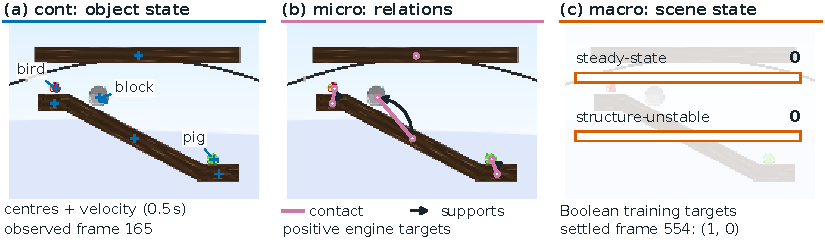
\includegraphics[width=\linewidth]{figures/fig_description_levels.pdf}
\caption{\textbf{Three description levels on one real frame.} A NovPhy frame during the cascade, described at each level $\alpha$. (a) $\textsf{cont}$: each object's centre and velocity. (b) $\textsf{micro}$: objects in contact (lines) and support relations (arrows, from supporter to supported). (c) $\textsf{macro}$: two scene predicates, both false here; once the scene settles (frame 554), steady-state becomes true. All panels show engine states and the engine labels used as training targets, not model outputs.}
\label{fig:levels}
\end{figure}

% ==== BRIEF §3 ¶3 (request-selection problem) =========================================
% [中] 定位：创新 3 的形式基础。先写请求条件化 rollout（策略在可行请求上取 argmax，按 Δ 推进，κ=0 停止；carrier 帧上的
%      semi-MDP，环境仍是引擎步 MDP），再写"好的请求日程"的目标：时长加权的单步预测误差加 λ 倍归一化计算量；目标需要观测到的
%      未来，只在训练轨迹上有定义，策略只能看 (ẑ_k, a, κ_k)；解法（DP + 蒸馏）在 §4。
%      主张：G(r_{1:J}) = Σ_j [Δ(r_j)·(1/d)‖F_θ(z̃_{k_j},a,r_j)−z_{k_j+Δ(r_j)}‖² + λ·MAC(r_j)]，d=236；MAC(r) = 一次转移（含策略）的线性
%            MAC 与仅预测器的 (15,cont) 转移之比。
%      证据：CH:216-239（adaptive_rollout：argmax、elapsed+=delta）；CH:142-155（Δ>remaining 掩码）；CH:158-176（linear_macs，
%            controller=True 加策略 MAC）；CH:179-212（:190 分母、:196 维度平均、:197 代价）；matched_dynamics.py:158-180。
%      手法与边界：问题与解法分开；误差项是从上下文出发的单步误差，不是递归端点误差；不写效果。
% [EN] Role: formal basis of innovation 3: the request-conditioned rollout (argmax over feasible requests, advance by
%      Δ, stop at κ = 0; a semi-MDP over carrier frames while the environment stays an engine-step MDP), then the
%      objective a good schedule minimizes: duration-weighted one-step error plus λ times normalized compute. The
%      objective needs the observed future, so it exists on training trajectories only; the policy sees (ẑ_k, a, κ_k).
%      Section 4 gives the solution (DP plus distillation).
%      Evidence: CH:216-239; CH:142-155; CH:158-176; CH:179-212; matched_dynamics.py:158-180.
%      Craft/Boundaries: problem separated from solution; the error is a one-step error from the context, not a
%      recursive endpoint error; no effect claims.
% ==== /BRIEF ==========================================================================
Given a launch $a$ and a rollout endpoint of $K$ carrier frames, the model rolls forward from $\hat z_0=z_0$. At frame $k$, with $\kappa_k=K-k$ frames remaining, a request policy $\pi_\psi$ issues one feasible request and the model advances by its horizon:
\begin{align}
r_k&=\argmax_{r\in\mathcal{R}:\ \Delta(r)\le\kappa_k}\ \pi_\psi(r\mid\hat z_k,a,\kappa_k),
\label{eq:policy}\\
\hat z_{k+\Delta(r_k)}&=F_\theta(\hat z_k,a,r_k),\qquad \kappa_{k+\Delta(r_k)}=\kappa_k-\Delta(r_k).
\label{eq:rollout}
\end{align}
The rollout stops at $\kappa=0$. Its steps last $\Delta(r_k)$ frames, so the rollout is a semi-MDP over carrier frames with state $(\hat z_k,\kappa_k)$ and the requests as actions, while the environment stays the MDP of Equation~\ref{eq:mdp}. A good schedule predicts accurately at little compute. On a training trajectory $z_{0:L}$ with launch $a$, a schedule $r_{1:J}$ whose horizons sum to $L$ costs
\begin{equation}
G(r_{1:J})=\sum_{j=1}^{J}\Big[\Delta(r_j)\,\tfrac1d\big\lVert F_\theta(\tilde z_{k_j},a,r_j)-z_{k_j+\Delta(r_j)}\big\rVert_2^2+\lambda\,\mathrm{MAC}(r_j)\Big],
\label{eq:objective}
\end{equation}
where step $j$ starts at frame $k_j$ from the context carrier $\tilde z_{k_j}$, $d=236$, and $\mathrm{MAC}(r)$ is the multiply-accumulate count of one transition under $r$, policy included, relative to the continuous transition at $\Delta=15$. The error term is the duration-weighted error of one prediction from its context. Equation~\ref{eq:objective} needs the observed future, so it is defined on training trajectories only, whereas $\pi_\psi$ must choose from $(\hat z_k,a,\kappa_k)$ alone. Section~\ref{sec:mth:model} solves Equation~\ref{eq:objective} by dynamic programming and distills the solutions into $\pi_\psi$.

% ==== BRIEF §3 ¶4 (from predictions to decisions) =====================================
% [中] 定位：把预测接到决策：候选集上的想象与计数代价 Ĵ、argmin 选择、引擎结局 y；定义排序 AUC（teaser 用到的术语）；
%      声明核心比较：同一 checkpoint、候选、端点与代价下，逐预测选择 vs 固定请求，r† 为在其他发射集上平均 AUC 最好的固定请求。
%      主张：Ĵ=1000·Σ pig 存在 + Σ block 存在（截断到 [0,1]）；平局取低 ordinal；y 不进入训练与排序；
%            AUC(s)=P[Ĵ(a+)<Ĵ(a−)]+½P[相等]，仅在 C(s) 同时含成功与失败时有定义。
%      证据：TO:31-42（计数代价）；TO:3-4（真实结局不进入评估器与规划器）；scripts/run_lookahead_control.py:9（平局规则）；
%            scripts/run_tau_ad_within_checkpoint.py:1-16（18 个日程、同一端点 225、同一代价）；issue-96 plan.json（F* 交叉拟合：
%            在其他三个发射集上平均 AUC 最好）；cell AUC 平局计 0.5。
%      手法与边界：一式定义、一句比较；发射集细节在 §5；无结果数字。
% [EN] Role: connects predictions to decisions: imagination over candidates with the count cost Ĵ, argmin selection,
%      engine outcome y; defines the ordering AUC used in the teaser; states the core comparison: per-prediction choice
%      against fixed requests on the same checkpoint, candidates, endpoint and cost, with r† the fixed request whose
%      mean AUC is best on the other launch sets.
%      Evidence: TO:31-42; TO:3-4; scripts/run_lookahead_control.py:9; scripts/run_tau_ad_within_checkpoint.py:1-16;
%      issue-96 plan.json (cross-fit F*); ties count one half in the cell AUC.
%      Craft/Boundaries: one defining equation per object; launch-set details live in Section 5; no result numbers.
% ==== /BRIEF ==========================================================================
At a decision state $s$, the agent imagines every launch in a candidate set $\mathcal{C}(s)$ by Equation~\ref{eq:rollout} and reads a task cost on the predicted endpoint carrier $\hat z_K$:
\begin{equation}
\hat J(a)=1000\sum_{i\in\mathcal{I}_{\mathrm{pig}}}\bar p_i(\hat z_K)+\sum_{i\in\mathcal{I}_{\mathrm{block}}}\bar p_i(\hat z_K),\qquad
\hat a=\argmin_{a\in\mathcal{C}(s)}\hat J(a),
\label{eq:select}
\end{equation}
where $\bar p_i(z)$ is slot $i$'s presence entry clipped to $[0,1]$, and $\mathcal{I}_{\mathrm{pig}}$ and $\mathcal{I}_{\mathrm{block}}$ index the target (pig) and block slots. Ties go to the lower candidate ordinal. The engine outcome $y(s,a)\in\{0,1\}$ is $1$ when the engine, executing $a$ from $s$, removes the target at the first shot; it enters neither training nor ranking. Because the agent acts on the order of $\hat J$, we score that order by the \emph{ordering AUC}, the probability that a successful launch is predicted to cost less than a failed one:
\begin{equation}
\mathrm{AUC}(s)=\Pr\big[\hat J(a^{+})<\hat J(a^{-})\big]+\tfrac12\Pr\big[\hat J(a^{+})=\hat J(a^{-})\big],\qquad y(s,a^{+})=1,\ y(s,a^{-})=0,
\label{eq:auc}
\end{equation}
with $a^{+}$ and $a^{-}$ drawn uniformly from $\mathcal{C}(s)$, defined when $\mathcal{C}(s)$ contains both outcomes. To isolate the request schedule, we compare $\pi_\psi$ with fixed requests ($r_k\equiv r$) on the same checkpoint, candidates, endpoint and cost; the fixed-request reference $r^{\dagger}$ is the request with the best mean AUC on the other launch sets.

% ==== BRIEF §4 HEAD (Method) ==========================================================
% [中] 定位：实现 §3 的对象，不重复 §1/§3 已说过的内容：§3 定义请求、共享潜变量与请求选择目标；§4 只给出实现（编码器、
%      请求条件化预测器、训练、策略的解法、只按时距条件化的基线）。超参数移到 Appendix sec:app:impl。
% 卖点：一个联合请求编码调制整个主干；九个请求共享全部权重；每次调用的计算量几乎与 α 无关。
%      主张：只描述已实现、已评估的部件；每个常数都有代码出处。
%      证据：CH = world_model/training/cnn_hybrid.py；PR = world_model/model/predictor.py；MD = world_model/training/matched_dynamics.py；
%            N1T = scripts/run_issue_77_n1_train.py；N1P = .local-artifacts/issue-77-n1-dynamics-v1/plan.json。
%      手法/边界：先总览，再部件；不得出现 TPR、GINE、SPSG、reliability gate、semantic embeddings；不得写 EMA 目标编码器；
%            不写控制器效果；不写两轴必须一起选；不重复 §3 的"同一空间、可随时切换""单步误差"与 §1 的"无 RL、无任务结局标签"。
% [EN] Role: implements the objects of Section 3 without repeating Sections 1 and 3: Section 3 defines requests, the
%      shared latent and the request-selection objective; Section 4 gives only the implementation (encoder,
%      request-conditioned predictor, training, the policy's solution method, the horizon-only baseline).
%      Hyperparameters move to Appendix sec:app:impl.
% Pitch: one joint request code modulates the whole trunk; the nine requests share every weight; per-call compute is
%      nearly independent of α.
%      Craft/Boundaries: overview first, then parts. No proposal-only components, no EMA target encoder, no controller
%      benefit; do not restate Section 3 ("same space, switch at any step", "one-step error") or Section 1 ("no RL,
%      no task-outcome labels").
% ==== /BRIEF ==========================================================================
\section{Method}
\label{sec:mth:model}

%!TEX root = iclr2026_conference.tex
% ==== BRIEF FIG (fig:mth:arch) ====
% [中] 定位：方法总览；一个按请求条件化的预测器服务全部九种 (Delta, alpha) 请求，
%      而非九个模型。面向 JEPA / world-model 读者，突出逐次预测可变的粒度。
%      主张：蓝色主路从真实 RGB 经冻结 CNN 对象槽编码器到同一连续 carrier；青绿色
%      请求码调制全部三个 FiLM 块；micro/macro 的软谓词经无偏置适配器在块前注入。
%      递归只更新 carrier，直到端点；按预测端点任务代价最小化选择候选 launch。
%      证据：world_model/training/cnn_hybrid.py:18-22,33-86（九请求、236 维、384 宽、
%      三块、残差、软读出与块前适配器）；world_model/model/predictor.py:218-274
%      （sinusoidal Delta + alpha embedding 联合码、零初始化 scale/shift）。
%      world_model/training/cohort_v2_visual_parser.py:272-291（CNN 对象槽 parser）；
%      world_model/data/deployment_temporal.py:553-554,599-621,680-719,734-750
%      （当前帧及可选前帧、无梯度解析、2+18x13 carrier）；
%      scripts/run_issue_70_parser_repair.py:96-98,464-472（维度与冻结检查点装载）。
%      policy 实际为 236 carrier + 5 action + 1 remaining = 242 -> 128 -> 9，
%      remaining 为 min(remaining,60)/60，越界请求被 mask：
%      world_model/training/matched_dynamics.py:91-104,132-154。
%      action = (drag_x/480,drag_y/480,release/1000,tap/1000,1)：
%      scripts/run_lookahead_control.py:588-591；端点评分及最小值选择：
%      scripts/run_tau_ad_within_checkpoint.py:401-458；run_lookahead_control.py:659-664。
%      训练：world_model/training/cnn_hybrid.py:89-139（局部 teacher-forced MSE、
%      递归 MSE、0.1 symbolic BCE、0.01 carrier bound）；
%      scripts/run_issue_77_n1_train.py:228-260,289-303,451-452,480-498,516-563
%      （engine 标签、冻结编码目标、九请求轮转、DP 标签 CE 与第二轮 DAgger 式聚合）。
%      DP 步代价 = Delta*(1/236)||F_theta(z,a,r)-z_future||^2
%      + 1e-4*(MAC_F(r)+MAC_pi)/MAC_F(15,continuous)，再加后继 value；
%      world_model/training/matched_dynamics.py:107-111,157-184。
%      手法与边界：真实图仅等比例裁剪 figures/source/001_common_decision.png；
%      槽堆栈是 carrier 图标，着色格为示意选择；训练灰色虚线带与运行时路径隔开。
%      JEPA-style latent predictor over a frozen object-slot encoder；无 EMA target encoder，
%      无 stop-gradient target branch。policy 仅在 decision-only imagined rollouts 受评，
%      从未闭环执行；scripts/run_tau_ad_within_checkpoint.py:12-17,845-855。
% [EN] Role: Method overview for JEPA / world-model readers: one shared predictor serves
%      nine requests, with granularity selected anew for each imagined prediction.
%      Claim: RGB becomes a frozen object-slot carrier (blue); the joint request code
%      modulates all three FiLM blocks (teal); micro/macro soft readouts feed back through
%      bias-free adapters before the blocks (violet/orange). Every mode advances the same
%      continuous carrier. Rollouts rank candidate launches by predicted endpoint task cost.
%      Evidence: world_model/training/cnn_hybrid.py:18-86,89-139;
%      world_model/model/predictor.py:218-274; world_model/training/cohort_v2_visual_parser.py:272-291;
%      world_model/data/deployment_temporal.py:553-554,599-621,680-719,734-750;
%      scripts/run_issue_70_parser_repair.py:96-98,464-472 (frozen encoder/carrier).
%      Policy input is 236 carrier + 5 action + 1 normalized remaining, not carrier alone:
%      world_model/training/matched_dynamics.py:91-104. Action and minimum-cost selection:
%      scripts/run_lookahead_control.py:588-591,659-664. Recursive endpoint scoring:
%      scripts/run_tau_ad_within_checkpoint.py:401-458.
%      Local + recursive MSE, 0.1 engine-label symbolic BCE and 0.01 bound:
%      world_model/training/cnn_hybrid.py:89-139; scripts/run_issue_77_n1_train.py:228-260,289-303.
%      Round-robin, CE on DP labels, and second-round DAgger-style aggregation:
%      scripts/run_issue_77_n1_train.py:451-452,480-498,516-563.
%      DP step cost is Delta*MSE + 1e-4*(predictor MACs + policy MACs)/continuous-15
%      predictor MACs, plus continuation value; world_model/training/matched_dynamics.py:107-111,157-184.
%      Craft: 5.5 x 2.6 in; >=7 pt base text; three visual lanes; policy inputs drawn (carrier z_k in blue,
%      launch a in ink; kappa_k named in-box); real aspect-preserving frame crop; editable SVG text, embedded PDF fonts.
%      Caption opens with bold "Model overview." (owner directive); the three disclaimers are one sentence.
%      The selected request is schematic, not an observed decision. This is a JEPA-style
%      latent predictor over a frozen object-slot encoder, with no EMA or stop-gradient
%      target branch. Policy evaluation was decision-only, never closed-loop:
%      scripts/run_tau_ad_within_checkpoint.py:12-17,845-855. No proposal-only modules are drawn.
% ==== /BRIEF ====
\begin{figure}[t]
  \centering
  
\includegraphics[width=\linewidth]{fig_model_overview}
  \caption{\textbf{Model overview.} One request-conditioned predictor serves all nine $(\Delta,\alpha)$ requests. This JEPA-style latent predictor over a frozen object-slot encoder advances a continuous carrier (blue), receives request modulation (teal), and feeds soft predicates back only for micro/macro requests (violet/orange); training signals (bottom) are separate from runtime inputs. The highlighted cell is schematic; there is no EMA target encoder, and the policy was evaluated only in decision-only imagined rollouts, never in closed loop.}
  \label{fig:mth:arch}
\end{figure}


% ==== BRIEF §4 ¶1 (overview and the sense of JEPA-style) ==============================
% [中] 定位：四个部件与训练顺序；并一次说清在什么意义上是 JEPA 式的（原 ¶1 与 ¶7 合并）。
%      主张：E 冻结；F_θ 与两个读出头联合训练；π_ψ 在 F_θ 冻结后训练；潜空间预测、无像素解码器；目标是冻结编码器给出的观测
%            未来帧 carrier，没有 EMA 目标编码器与 stop-gradient 分支。
%      证据：N1T:415-474（train_cell）与 :502-583（train_control 载入冻结预测器）；CH:105-139、MD:72-88（目标为观测 carrier）；
%            world_model/model/jepa.py 与 ema.py 不在评估系统中使用。
%      手法与边界：三句；必须写 "JEPA-style"，不称完整 JEPA。
% [EN] Role: the four parts, the training order, and the one statement of the sense in which the model is JEPA-style
%      (former ¶1 and ¶7 merged).
%      Evidence: N1T:415-474 and :502-583; CH:105-139, MD:72-88 (targets are observed carriers); jepa.py / ema.py
%      unused by the evaluated systems.
%      Craft/Boundaries: three sentences; "JEPA-style", never a full JEPA.
% ==== /BRIEF ==========================================================================
The model has four parts (Figure~\ref{fig:mth:arch}): the frozen encoder $E$, the request-conditioned predictor $F_\theta$, two predicate heads, and the request policy $\pi_\psi$. $F_\theta$ and the heads train jointly, and $\pi_\psi$ trains afterwards with $F_\theta$ frozen. The predictor is JEPA-style in that it predicts future carriers in latent space without a pixel decoder; its targets are the frozen encoder's carriers of observed future frames, with no EMA target encoder or stop-gradient branch.

% ==== BRIEF §4 ¶2 (encoder and carrier) ===============================================
% [中] 定位：编码器与 carrier 的实现；不重复 §3 ¶2 的逐物体内容描述（存在、类别、位置、速度）。
%      主张：E 为小型 CNN object-slot 解析器，96×64 帧，18 个命名槽；一次性有监督训练后冻结；z=[g; f_1..f_18]，g 为是否有前一帧与
%            经过时间，每槽 13 维；速度来自与前一帧的差分（对应 Figure 3 的 "+ previous frame"）。
%      证据：scripts/run_issue_70_parser_repair.py:37-39、:111-112、:302-344；world_model/data/deployment_temporal.py:26-40、
%            :659-832，速度 :704-717。
%      手法与边界：一式两句；解析器是有监督的，不写成自监督。
% [EN] Role: implementation of the encoder and carrier, without repeating the per-object content listed in Section 3.
%      Evidence: run_issue_70_parser_repair.py:37-39, :111-112, :302-344; deployment_temporal.py:26-40, :659-832
%      (velocity :704-717).
%      Craft/Boundaries: one equation, two sentences; the parser is supervised.
% ==== /BRIEF ==========================================================================
\textbf{Encoder and carrier.} $E$ is a small CNN object-slot parser that reads the $96\times64$ agent frame into 18 named slots from a fixed vocabulary. It was trained once with supervised slot and predicate labels and stays frozen during all dynamics training. The carrier stacks two global entries $g$, whether a prior frame exists and the elapsed time, with 13 features per slot,
\begin{equation}
z=\big[g;\,f_1;\dots;f_{18}\big]\in\mathbb{R}^{2+18\cdot13}=\mathbb{R}^{236},
\label{eq:carrier}
\end{equation}
where each slot's velocity is its displacement from the prior frame.

% ==== BRIEF §4 ¶3 (request-conditioned predictor) =====================================
% [中] 定位：创新 2 的实现：联合请求编码以 FiLM / AdaLN-Zero 调制每个残差块；micro/macro 头读出 §3 的谓词并经无偏置 adapter
%      加到主干输入；每次调用的计算量几乎与 α 无关。
%      主张：c(r)=MLP([φ(Δ); e_α])，九个请求各得一套调制而非两轴之和；宽 384、3 个块；调制零初始化；micro 头输出 18×18 槽对的
%            contact 与 supports 概率，macro 头输出两个场景谓词，各带 availability；每步恰好一个 adapter（cont 无）；
%            每次调用 linear MAC：cont 1,432,448，micro 1,795,456（+25%），macro 1,464,704（+2%）。
%      证据：CH:18-22、:33-48、:50-73、:75-86；PR:218-274（PairConditioner、FiLMBlock，零初始化 :268-269）；
%            CH:158-176 linear_macs（2026-09-26 在 novphy 环境中重新运行得到上述 MAC 数与 1,837,690 参数）；
%            perez2018film、peebles2023scalable。
%      手法与边界：机制句在前，公式随后；不重复 §3"谓词回馈改变被推进内容""返回同一空间的 carrier"；不写符号动力学。
% [EN] Role: implementation of innovation 2: a joint request code FiLM/AdaLN-Zero-modulates every residual block; the
%      micro/macro heads read the predicates of Section 3 and a bias-free adapter adds them to the trunk input;
%      per-call compute is nearly independent of α.
%      Evidence: CH:18-22, :33-48, :50-73, :75-86; PR:218-274; CH:158-176 linear_macs (re-run 2026-09-26: MACs above,
%      1,837,690 parameters); perez2018film, peebles2023scalable.
%      Craft/Boundaries: mechanism sentence, then equations; do not restate Section 3's feedback and shared-space
%      sentences; no symbolic dynamics.
% ==== /BRIEF ==========================================================================
\textbf{Request-conditioned predictor.} $F_\theta$ is a residual MLP trunk of width 384 whose three blocks are all modulated by one code for the whole request. The code fuses sinusoidal features $\phi(\Delta)$ of the horizon with a learned embedding $e_\alpha$ of the description level in one MLP, so each of the nine requests receives its own modulation rather than a sum of a horizon term and a description term. Modulation is FiLM-style \citep{perez2018film}, with scale and shift initialized at zero as in AdaLN-Zero \citep{peebles2023scalable}, so training starts from an unmodulated trunk:
\begin{align}
c(r)&=\mathrm{MLP}_c\big([\phi(\Delta);\,e_\alpha]\big),
\label{eq:code}\\
x^{(0)}&=W_{\mathrm{in}}\,[\hat z_k;\,a]+\mathbf{1}[\alpha\neq\textsf{cont}]\;U_\alpha\,h_\alpha(\hat z_k),
\label{eq:input}\\
x^{(\ell)}&=x^{(\ell-1)}+\mathrm{MLP}_\ell\Big(\mathrm{LN}\big(x^{(\ell-1)}\big)\odot\big(1+\gamma_\ell(c)\big)+\beta_\ell(c)\Big),\qquad \ell=1,2,3,
\label{eq:film}\\
\hat z_{k+\Delta}&=\hat z_k+W_{\mathrm{out}}\,\mathrm{LN}\big(x^{(3)}\big),
\label{eq:residual}
\end{align}
where $a\in\mathbb{R}^5$ encodes the launch. The head $h_{\textsf{micro}}$ outputs contact and support probabilities over $18\times18$ slot pairs, and $h_{\textsf{macro}}$ outputs the two scene predicates, each with an availability output; the bias-free adapter $U_\alpha$ adds them to the trunk input, and a $\textsf{cont}$ request runs no head. Per call, a $\textsf{micro}$ request costs 25\% more multiply-accumulates than a $\textsf{cont}$ request and a $\textsf{macro}$ request 2\% more, so the compute of a schedule is set mainly by how many calls it makes, that is, by its horizons.

% ==== BRIEF §4 ¶4 (training) ==========================================================
% [中] 定位：一套权重服务九个请求的实现事实（轮转）在前；一行损失；标签来源；单位差异披露。超参数在附录。
%      主张：每次更新训练一个请求 r=R[u mod 9]，无课程；损失 = 局部 MSE + 递归 MSE（无 teacher forcing 的 ẑ_j）+ 0.1×符号项
%            （预测 carrier 与观测上下文各一次；ℓ_cont≡0）+ 0.01×carrier 界（|z|>2）；M≤4 步，k_j=jΔ≤L≤60；
%            谓词标签来自引擎（micro：由物体记录投影的接触与支撑；macro：稳定事件与支撑集变化），不可用帧掩码；
%            2,409 条拟合 lineage 中 2,400 条基础语料为帧距 1，Δ 以引擎步计，其余 N1 分片为 §3 的 50 步帧。
%      证据：CH:89-139（损失与权重）；N1T:140-148、:451-452（PAIRS[step%9]）；N1T:23-32、:228-249（标签来源）；N1T:14-19 与
%            scripts/run_issue_71_hybrid_readiness.py:139-140（单位差异）；N1P training.fit_lineages=2409。
%      手法与边界：一式一段；如实披露单位差异，不加推论；不写课程学习。
% [EN] Role: the fact that makes one set of weights serve nine requests (round-robin) comes first; the loss in one
%      line; label sources; the unit disclosure. Hyperparameters live in the appendix.
%      Evidence: CH:89-139; N1T:140-148, :451-452; N1T:23-32, :228-249; N1T:14-19 and run_issue_71_hybrid_readiness.py:139-140;
%      N1P training.fit_lineages = 2409.
%      Craft/Boundaries: one equation; disclose the unit difference plainly; no curriculum.
% ==== /BRIEF ==========================================================================
\textbf{Training.} Each update trains one request, cycling $r=\mathcal{R}[u \bmod 9]$ at update $u$ without a curriculum, so all nine requests share every weight of the trunk. For a training window of observed carriers $z_{0:L}$ ($L\le60$) with launch $a$, the loss unrolls $M\le4$ steps of horizon $\Delta$ ending at $k_j=j\Delta\le L$:
\begin{equation}
\mathcal{L}(\theta;r)=\frac1M\sum_{j=1}^{M}\Big[\mathrm{mse}\big(F_\theta(z_{k_{j-1}},a,r),z_{k_j}\big)+\mathrm{mse}\big(\hat z_j,z_{k_j}\big)+\lambda_{\mathrm{sym}}\,\ell_\alpha^{(j)}+\lambda_{\mathrm{bd}}\,b(\hat z_j)\Big],
\label{eq:loss}
\end{equation}
where $\hat z_0=z_0$ and $\hat z_j=F_\theta(\hat z_{j-1},a,r)$ rolls without teacher forcing, $\mathrm{mse}(x,x')=\tfrac1d\lVert x-x'\rVert_2^2$, $b$ penalizes carrier entries beyond $\pm2$, $\lambda_{\mathrm{sym}}=0.1$ and $\lambda_{\mathrm{bd}}=0.01$. The symbolic term $\ell_\alpha^{(j)}$ is a masked binary cross-entropy of head $\alpha$ on the predicted carrier and on the observed context, and $\ell_{\textsf{cont}}\equiv0$. Its labels come from the engine: contact and support relations projected from the captured object records for $\textsf{micro}$, and stability events and support-set changes for $\textsf{macro}$. Of the 2,409 training lineages, the 2,400 of the base corpus are captured at every engine step, so there $\Delta$ counts engine steps rather than the 50-step frames of the N1 captures.

% ==== BRIEF §4 ¶5 (request policy: the solution) ======================================
% [中] 定位：§3 目标 eq:objective 的解法：逆向 DP 求最优日程，交叉熵蒸馏，DAgger 式第二轮；不重复 §3 的误差项性质与 §1 的
%      "无 RL、无任务结局标签"。
%      主张：π_ψ 为 242→128→9 MLP，输入 [ẑ_k; a; min(κ_k,60)/60]，Δ>κ_k 的 logit 置 −∞；λ=1e-4；平局取 R 的固定顺序；
%            第一轮上下文为观测 carrier，第二轮为第一轮策略自身 rollout 访问到的 carrier，标签对同一观测目标重算，两轮合并训练。
%      证据：CH:142-155（结构、掩码、/60）；CH:179-212（trajectory_labels）；N1T:480-499（第二轮上下文）；N1T:559-563（合并与
%            交叉熵）；ross2011dagger 不在 bib 中，故不引用，只写 "DAgger-style"。
%      手法与边界：两式一段；策略只在 decision-only 想象 rollout 中评估（§5 写明）；不写效果。
% [EN] Role: the solution of Section 3's objective: a backward DP for the optimal schedule, cross-entropy distillation,
%      a DAgger-style second round; no restatement of the error-term property (Section 3) or of "no RL" (Section 1).
%      Evidence: CH:142-155; CH:179-212; N1T:480-499; N1T:559-563.
%      Craft/Boundaries: two equations; no effect claims.
% ==== /BRIEF ==========================================================================
\textbf{Request policy.} $\pi_\psi$ is an MLP ($242\to128\to9$) on $[\hat z_k;\,a;\,\min(\kappa_k,60)/60]$ whose logits for requests with $\Delta>\kappa_k$ are set to $-\infty$. With $F_\theta$ frozen, a backward dynamic program finds the schedule that minimizes Equation~\ref{eq:objective} on each training window, and $\pi_\psi$ is trained by cross-entropy on its choices. With $g_k(r)$ the summand of Equation~\ref{eq:objective} for a step that starts at frame $k$, and $\lambda=10^{-4}$,
\begin{align}
V(k)&=\min_{r\in\mathcal{R}:\ k+\Delta(r)\le L}\Big[g_k(r)+V\big(k+\Delta(r)\big)\Big],\qquad V(L)=0,
\label{eq:dp}\\
\mathcal{L}_\pi(\psi)&=-\sum_{k<L}\log\pi_\psi\big(r^{\star}_k\mid\tilde z_k,a,L-k\big),
\label{eq:distill}
\end{align}
where $r^{\star}_k$ is the minimizer in Equation~\ref{eq:dp}, with ties broken by a fixed order of $\mathcal{R}$. In round 1 the contexts $\tilde z_k$ are the observed carriers. Round 2 is DAgger-style: it takes as contexts the carriers that the round-1 policy visits in its own rollout of the window, recomputes the labels against the same observed targets, and trains on both rounds' labels.

% ==== BRIEF §4 ¶6 (horizon-only baseline) =============================================
% [中] 定位：只按时距条件化的纯连续基线；说明它在正文中的两个用途（Figure 1 b1 的连续模型；§1 的 horizon-only adaptive
%      baseline），并如实说明计算对比所用的训练轮次。
%      主张：同一主干与损失（无符号项）；c(Δ)=MLP(φ(Δ))；无读出头、adapter、α 嵌入，只接受 cont；宽 456 为最接近 hybrid 参数量的
%            宽度（1,862,396 对 1,837,690）；其策略在三个连续请求上选择，由同一 DP 以自身计算量标注；两模型共享种子、minibatch 与
%            更新预算，每次更新训练同一 Δ；计算对比使用同一配方只在 2,400 条基础语料上的训练（issue-74，600 条策略 lineage）。
%      证据：MD:15-46、:57-69、:72-88、:158-184；N1P capacity（1,862,396、456、1,837,690）；issue-74-matched-dynamics-v1/plan.json
%            training（fit_lineages 2400、controller_lineages 600）与 readiness.json capacity；issue-77-n1-diagnostic-v1/summary.json
%            （continuous_h1/h5/h15 为该基线在固定 Δ 下的曲线）。
%      手法与边界：参数量匹配不是算力匹配（附录）；不写效果。
% [EN] Role: the continuous-only, horizon-conditioned baseline; names its two uses in the main text (the continuous model
%      of Figure 1(b1); the horizon-only adaptive baseline of Section 1) and states which training the compute comparison
%      uses.
%      Evidence: MD:15-46, :57-69, :72-88, :158-184; N1P capacity; issue-74 plan.json training (2,400 fitting and 600
%      policy lineages) and readiness.json capacity; issue-77 diagnostic summary (continuous_h* curves).
%      Craft/Boundaries: parameter matching is not compute matching (appendix); no effect claims.
% ==== /BRIEF ==========================================================================
\textbf{Horizon-only baseline.} The baseline $\theta^{\mathrm{con}}$ is the continuous-only model of Figure~\ref{fig:teaser}(b1) and, with its own policy, the horizon-only adaptive baseline of Section~\ref{sec:introduction}. It uses the trunk of Equations~\ref{eq:film}--\ref{eq:residual} and the loss of Equation~\ref{eq:loss} without symbolic terms, but its code depends on the horizon alone, $c(\Delta)=\mathrm{MLP}_c(\phi(\Delta))$; it has no heads, adapters or description embedding and accepts only $\textsf{cont}$. Its trunk width of 456 is the width nearest the hybrid's parameter count (1,862,396 against 1,837,690). Its policy chooses among the three continuous requests and is labelled by the same dynamic program with its own compute counts. Both models share seeds, minibatches and update budget, and at each update the baseline trains the same $\Delta$ as the hybrid. The compute comparison uses a training of both models by the same recipe on the base corpus alone (Appendix~\ref{sec:app:impl}).

% ==== BRIEF §5 HEAD (Experimental Setup) ==============================================
% [中] 定位：为 §1 的三条发现给出最小的评测设置：数据与模型、滚动误差、候选发射排序、计算对比；最后一段交代统计与范围。
%      不重复 §3 已定义的 Ĵ、y、排序 AUC 与 r†，只引用；不出现成员 ID、类型编号、ticket 编号。
% 卖点：每个数字都来自冻结的计划与保留的 artifact；三个 benchmark 分开报告。
%      证据：见各段 BRIEF。
%      手法与边界：短；区间只作描述；策略只在 decision-only 想象 rollout 中评估；不写泛化。
% [EN] Role: the minimum setup behind the three findings of Section 1: data and models, rollout error, ranking of
%      candidate launches, the compute comparison, then one paragraph on statistics and scope. Reuses, never restates,
%      Ĵ, y, ordering AUC and r† from Section 3; no member IDs, type codes or ticket numbers.
%      Craft/Boundaries: short; intervals descriptive; decision-only; no generalization claim.
% ==== /BRIEF ==========================================================================
\section{Experimental Setup}
\label{sec:mth:protocol}

% ==== BRIEF §5 ¶1 (benchmarks and models) =============================================
% [中] 定位：三个 benchmark 与各自的模型。
%      主张：NovPhy 上用 §4 的冻结解析器读渲染帧；CLEVRER 与 Physion-Dominoes 没有智能体动作，carrier 由发布的物体标注按同一
%            236 维布局构造，两类模型在其上从头训练、同一结构与更新预算；macro 谓词只在 NovPhy 上有；三个种子；逐 benchmark 报告。
%      证据：scripts/run_clevrer_boundary_replication.py 与 scripts/run_third_family_boundary_replication.py 文档串（"retrained from
%            scratch on the frozen … annotation-derived carrier"，"three paired seeds, 9000 identical updates"，"macro arm is
%            unsupported"）；两者 summary.json representation.carrier（"unchanged issue-71 236-value layout"）；
%            issue-77-n1-dynamics-v1/plan.json seeds [20260908, 20260909, 20260910]。
%      手法与边界：不写 CLEVRER/Physion 上有感知；不合并三个 benchmark。
% [EN] Role: the three benchmarks and their models.
%      Evidence: docstrings of run_clevrer_boundary_replication.py and run_third_family_boundary_replication.py; their
%      summary.json representation.carrier; issue-77 plan seeds.
%      Craft/Boundaries: no perception claim on CLEVRER/Physion; benchmarks never pooled.
% ==== /BRIEF ==========================================================================
\textbf{Benchmarks and models.} On NovPhy \citep{pinto2024novphy} we use levels with normal physics, and the frozen encoder of Section~\ref{sec:mth:model} parses the rendered frames. CLEVRER \citep{yi2020clevrer} and Physion-Dominoes \citep{bear2021physion} have no agent actions; there we build the carrier from the released object annotations in the same 236-value layout and train both the hybrid and the baseline from scratch with the same architecture and update budget. Macro predicates exist only on NovPhy, so the other two benchmarks use $\textsf{cont}$ and $\textsf{micro}$. Every model is trained with three seeds, and each benchmark is reported separately.

% ==== BRIEF §5 ¶2 (rollout error) =====================================================
% [中] 定位：发现 1（Figure 1 b1）的测量。
%      主张：从一个观测 carrier 出发，按固定请求 (Δ, cont) 递归展开、不重置，报告预测物体位置对观测位置的均方误差；NovPhy 上起点为
%            四个留出关卡的发射帧、每关 13 个候选发射，端点至 225 carrier 帧；另两个 benchmark 为每种子 48 个（场景, 上下文）单元，
%            端点至 120 帧。
%      证据：issue-77-n1-diagnostic-v1/summary.json definitions（recursive "no truth resets"；field_masks position[5,6]；
%            membership held-out；times）、inventory evaluable_states=4、headroom candidates=13；issue-79 / issue-84 summary.json
%            membership eval_units_per_seed=48、12 个场景/试次；build_scene_figures.py 所用端点 (15..225) 与 (15..120)。
%      手法与边界：600 端点右删失，不用；不写 "held-out 泛化"。
% [EN] Role: the measurement behind finding 1 (Figure 1(b1)).
%      Evidence: issue-77 diagnostic definitions, inventory and headroom; issue-79/84 membership; teaser builder endpoints.
%      Craft/Boundaries: the right-censored 600 endpoint is not used; no generalization claim.
% ==== /BRIEF ==========================================================================
\textbf{Rollout error.} From one observed carrier, a fixed request $(\Delta,\textsf{cont})$ is applied recursively, each prediction feeding the next without resets, and we report the mean squared error of the predicted object positions against the observed ones. On NovPhy the rollouts start at the launch frame of four held-out levels, one per candidate launch (13 per level), and run to 225 carrier frames; on CLEVRER and Physion-Dominoes they start from 48 context frames in 12 evaluation scenes and run to 120 frames.

% ==== BRIEF §5 ¶3 (ranking candidate launches) ========================================
% [中] 定位：发现 2 与发现 3 前半（Figure 1 b2）的测量。
%      主张：决策状态 = 一个 NovPhy 关卡加一组候选发射，每个候选在引擎中执行一次得到 y；四个发射集（角度扫描 9–13、另一组 11 个角度、
%            4×4 拖拽网格 16、角度×力度 20 且力度超出训练范围）覆盖同一批 15 个关卡；只有同时含成功与失败的关卡计分（每集 7–14 个）；
%            每个候选从关卡发射帧 carrier 想象到 225 帧；逐关卡、逐种子算排序 AUC；在同一 hybrid checkpoint 上比较策略与九个固定请求；
%            r† 交叉拟合，另报每集事后最佳固定请求。
%      证据：issue-96 plan.json universe.inventories、mixed_rule 与 mixed_members（grid 14、offset 9、angle 7、power 8）、
%            held_identical.endpoint=225 与 anchors；scripts/run_tau_ad_within_checkpoint.py:1-16、:778-780（cross_fit）；
%            findings.md 列 F_hindsight。
%      手法与边界：发射集是候选生成方式而非选择方法；力度集在训练范围外；不在此给结果。
% [EN] Role: the measurement behind finding 2 and the first half of finding 3 (Figure 1(b2)).
%      Evidence: issue-96 plan.json (inventories, mixed rule and members, endpoint, anchors); run_tau_ad_within_checkpoint.py
%      (cross-fit); findings.md (F_hindsight column).
%      Craft/Boundaries: launch sets generate candidates, they are not selection methods; no results here.
% ==== /BRIEF ==========================================================================
\textbf{Ranking candidate launches.} A decision state is a NovPhy level with a set of candidate launches, each executed once in the engine to record its outcome $y$. Four launch sets vary the launch differently: a sweep of launch angles (9--13 candidates), a sweep of 11 other angles, a $4\times4$ grid of drag vectors, and a sweep of angle and launch power whose powers lie outside the training range (20 candidates). The sets cover the same 15 levels, and a level is scored in a set only when the set holds both a success and a failure, which leaves 7--14 levels per set. Every candidate is imagined from the level's launch-frame carrier to 225 carrier frames, and the ordering AUC (Equation~\ref{eq:auc}) is computed per level and seed. On the same hybrid checkpoints we compare the request policy with all nine fixed requests: the cross-fitted reference $r^\dagger$ of Section~\ref{sec:mth:setting} and, as an upper reference, the fixed request that is best on each set in hindsight.

% ==== BRIEF §5 ¶4 (compute) ===========================================================
% [中] 定位：发现 3 后半（两轴选择以约三分之一计算量匹配只调时距的基线）的测量。
%      主张：200 个开发状态、每状态 12 个候选、端点 225、三个种子；每个系统按预测代价选择；所选发射按引擎在捕获窗口末实现的计数代价
%            的归一化遗憾计分；计算量 = 每个候选-状态的全部预测器与策略调用的线性 MAC；训练轮次见 Appendix sec:app:impl。
%      证据：issue-74-matched-dynamics-v1/plan.json development（states 200、candidates 12、endpoint 225、role calibration）；
%            scripts/run_issue_72_matched_grid.py:264-282（normalized_regrets 基于 realized_count_cost，平局取低序号）；
%            readiness.json compute.accounting（linear MACs，training_compute_matched=false）。
%      手法与边界：这些状态也用于选择基线策略（selection_optimism=true），在结果中写明；训练算力未匹配。
% [EN] Role: the measurement behind the second half of finding 3.
%      Evidence: issue-74 plan development block; run_issue_72_matched_grid.py:264-282; readiness.json compute.
%      Craft/Boundaries: the same states also select the baseline's policy (reported with the result); training compute
%      is not matched.
% ==== /BRIEF ==========================================================================
\textbf{Compute.} The comparison with the horizon-only baseline uses 200 development states with 12 candidate launches each, rolled to 225 carrier frames, and the three seeds of the training in Appendix~\ref{sec:app:impl}. Each system chooses the launch of lowest predicted cost; the choice is scored by its regret in the count cost that the engine realizes at the end of the capture window, normalized per state to $[0,1]$, and compute is the linear multiply-accumulates of all predictor and policy calls per candidate and state.

% ==== BRIEF §5 ¶5 (statistics and scope) ==============================================
% [中] 定位：一次交代统计与范围，替代旧的注册状态段与闭环范围段。
%      主张：每项分析在其计分结局产生前由冻结计划固定；区间为按关卡（或状态）聚类的百分位 bootstrap 95% 区间，只作描述；
%            策略只在 decision-only 想象 rollout 中评估，从未控制引擎；Appendix sec:app:protocol 给出计划与注册细节。
%      证据：issue-96 plan.json estimands.interval（member-clustered percentile bootstrap, 10000 draws）；issue-77 diagnostic
%            definitions.bootstrap（unit state，10000 draws）；issue-74 plan development.uncertainty；Appendix sec:app:protocol。
%      手法与边界：不写显著性；不列成员、类型编号、事后指定项的细目（在附录）。
% [EN] Role: statistics and scope in one paragraph, replacing the former registration-status and closed-loop paragraphs.
%      Evidence: issue-96 plan interval rule; issue-77 diagnostic bootstrap; issue-74 plan uncertainty; Appendix
%      sec:app:protocol.
%      Craft/Boundaries: no significance language; membership and post-hoc details stay in the appendix.
% ==== /BRIEF ==========================================================================
\textbf{Statistics and scope.} Each experiment ran under a plan frozen before the outcomes it scores existed (Appendix~\ref{sec:app:protocol}). Intervals are 95\% percentile bootstrap intervals that resample levels, scenes or states with all their seeds together, and are descriptive.
